\PassOptionsToPackage{unicode=true}{hyperref} % options for packages loaded elsewhere
\PassOptionsToPackage{hyphens}{url}
%
\documentclass[]{article}
\usepackage{lmodern}
\usepackage{amssymb,amsmath}
\usepackage{ifxetex,ifluatex}
\usepackage{fixltx2e} % provides \textsubscript
\ifnum 0\ifxetex 1\fi\ifluatex 1\fi=0 % if pdftex
  \usepackage[T1]{fontenc}
  \usepackage[utf8]{inputenc}
  \usepackage{textcomp} % provides euro and other symbols
\else % if luatex or xelatex
  \usepackage{unicode-math}
  \defaultfontfeatures{Ligatures=TeX,Scale=MatchLowercase}
\fi
% use upquote if available, for straight quotes in verbatim environments
\IfFileExists{upquote.sty}{\usepackage{upquote}}{}
% use microtype if available
\IfFileExists{microtype.sty}{%
\usepackage[]{microtype}
\UseMicrotypeSet[protrusion]{basicmath} % disable protrusion for tt fonts
}{}
\IfFileExists{parskip.sty}{%
\usepackage{parskip}
}{% else
\setlength{\parindent}{0pt}
\setlength{\parskip}{6pt plus 2pt minus 1pt}
}
\usepackage{hyperref}
\hypersetup{
            pdftitle={Oblig 2-STAT111},
            pdfauthor={Sigbjorn Fjelland},
            pdfborder={0 0 0},
            breaklinks=true}
\urlstyle{same}  % don't use monospace font for urls
\usepackage[margin=1in]{geometry}
\usepackage{color}
\usepackage{fancyvrb}
\newcommand{\VerbBar}{|}
\newcommand{\VERB}{\Verb[commandchars=\\\{\}]}
\DefineVerbatimEnvironment{Highlighting}{Verbatim}{commandchars=\\\{\}}
% Add ',fontsize=\small' for more characters per line
\usepackage{framed}
\definecolor{shadecolor}{RGB}{248,248,248}
\newenvironment{Shaded}{\begin{snugshade}}{\end{snugshade}}
\newcommand{\AlertTok}[1]{\textcolor[rgb]{0.94,0.16,0.16}{#1}}
\newcommand{\AnnotationTok}[1]{\textcolor[rgb]{0.56,0.35,0.01}{\textbf{\textit{#1}}}}
\newcommand{\AttributeTok}[1]{\textcolor[rgb]{0.77,0.63,0.00}{#1}}
\newcommand{\BaseNTok}[1]{\textcolor[rgb]{0.00,0.00,0.81}{#1}}
\newcommand{\BuiltInTok}[1]{#1}
\newcommand{\CharTok}[1]{\textcolor[rgb]{0.31,0.60,0.02}{#1}}
\newcommand{\CommentTok}[1]{\textcolor[rgb]{0.56,0.35,0.01}{\textit{#1}}}
\newcommand{\CommentVarTok}[1]{\textcolor[rgb]{0.56,0.35,0.01}{\textbf{\textit{#1}}}}
\newcommand{\ConstantTok}[1]{\textcolor[rgb]{0.00,0.00,0.00}{#1}}
\newcommand{\ControlFlowTok}[1]{\textcolor[rgb]{0.13,0.29,0.53}{\textbf{#1}}}
\newcommand{\DataTypeTok}[1]{\textcolor[rgb]{0.13,0.29,0.53}{#1}}
\newcommand{\DecValTok}[1]{\textcolor[rgb]{0.00,0.00,0.81}{#1}}
\newcommand{\DocumentationTok}[1]{\textcolor[rgb]{0.56,0.35,0.01}{\textbf{\textit{#1}}}}
\newcommand{\ErrorTok}[1]{\textcolor[rgb]{0.64,0.00,0.00}{\textbf{#1}}}
\newcommand{\ExtensionTok}[1]{#1}
\newcommand{\FloatTok}[1]{\textcolor[rgb]{0.00,0.00,0.81}{#1}}
\newcommand{\FunctionTok}[1]{\textcolor[rgb]{0.00,0.00,0.00}{#1}}
\newcommand{\ImportTok}[1]{#1}
\newcommand{\InformationTok}[1]{\textcolor[rgb]{0.56,0.35,0.01}{\textbf{\textit{#1}}}}
\newcommand{\KeywordTok}[1]{\textcolor[rgb]{0.13,0.29,0.53}{\textbf{#1}}}
\newcommand{\NormalTok}[1]{#1}
\newcommand{\OperatorTok}[1]{\textcolor[rgb]{0.81,0.36,0.00}{\textbf{#1}}}
\newcommand{\OtherTok}[1]{\textcolor[rgb]{0.56,0.35,0.01}{#1}}
\newcommand{\PreprocessorTok}[1]{\textcolor[rgb]{0.56,0.35,0.01}{\textit{#1}}}
\newcommand{\RegionMarkerTok}[1]{#1}
\newcommand{\SpecialCharTok}[1]{\textcolor[rgb]{0.00,0.00,0.00}{#1}}
\newcommand{\SpecialStringTok}[1]{\textcolor[rgb]{0.31,0.60,0.02}{#1}}
\newcommand{\StringTok}[1]{\textcolor[rgb]{0.31,0.60,0.02}{#1}}
\newcommand{\VariableTok}[1]{\textcolor[rgb]{0.00,0.00,0.00}{#1}}
\newcommand{\VerbatimStringTok}[1]{\textcolor[rgb]{0.31,0.60,0.02}{#1}}
\newcommand{\WarningTok}[1]{\textcolor[rgb]{0.56,0.35,0.01}{\textbf{\textit{#1}}}}
\usepackage{graphicx,grffile}
\makeatletter
\def\maxwidth{\ifdim\Gin@nat@width>\linewidth\linewidth\else\Gin@nat@width\fi}
\def\maxheight{\ifdim\Gin@nat@height>\textheight\textheight\else\Gin@nat@height\fi}
\makeatother
% Scale images if necessary, so that they will not overflow the page
% margins by default, and it is still possible to overwrite the defaults
% using explicit options in \includegraphics[width, height, ...]{}
\setkeys{Gin}{width=\maxwidth,height=\maxheight,keepaspectratio}
\setlength{\emergencystretch}{3em}  % prevent overfull lines
\providecommand{\tightlist}{%
  \setlength{\itemsep}{0pt}\setlength{\parskip}{0pt}}
\setcounter{secnumdepth}{0}
% Redefines (sub)paragraphs to behave more like sections
\ifx\paragraph\undefined\else
\let\oldparagraph\paragraph
\renewcommand{\paragraph}[1]{\oldparagraph{#1}\mbox{}}
\fi
\ifx\subparagraph\undefined\else
\let\oldsubparagraph\subparagraph
\renewcommand{\subparagraph}[1]{\oldsubparagraph{#1}\mbox{}}
\fi

% set default figure placement to htbp
\makeatletter
\def\fps@figure{htbp}
\makeatother


\title{Oblig 2-STAT111}
\author{Sigbjorn Fjelland}
\date{4/10/2020}

\begin{document}
\maketitle

Oppgave 1

Galton brukte fedres høyde for å estimere høyden til sønnen. I oppgaven
introduseres det at Galton også brukte også gjennomsnitts høyde på
forreldre (altså gjennomsnitt mellom mor og far). Videre er det gitt en
tabell med 11 snitthøyde til forreldre og høyde på tilhørende datter.

\begin{enumerate}
\def\labelenumi{\alph{enumi})}
\item
\end{enumerate}

\begin{verbatim}
I delspørsmål a skal vi lage ett spredningsplott for den gitte tabellen med snittøyde til forreldre satt opp mot datter. Tabellen kan tolkes som to vektorer som skal settes i plot med indeksering:
\end{verbatim}

\begin{Shaded}
\begin{Highlighting}[]
\NormalTok{Midparent <-}\StringTok{ }\KeywordTok{c}\NormalTok{(}\FloatTok{66.0}\NormalTok{, }\FloatTok{65.5}\NormalTok{, }\FloatTok{71.5}\NormalTok{, }\FloatTok{68.0}\NormalTok{, }\FloatTok{70.0}\NormalTok{, }\FloatTok{65.5}\NormalTok{, }\FloatTok{67.0}\NormalTok{, }\FloatTok{70.5}\NormalTok{, }\FloatTok{69.5}\NormalTok{, }\FloatTok{64.5}\NormalTok{, }\FloatTok{67.5}\NormalTok{)}
\NormalTok{Daughter <-}\StringTok{ }\KeywordTok{c}\NormalTok{(}\FloatTok{64.0}\NormalTok{, }\FloatTok{63.0}\NormalTok{, }\FloatTok{69.0}\NormalTok{, }\FloatTok{69.0}\NormalTok{, }\FloatTok{69.0}\NormalTok{, }\FloatTok{65.0}\NormalTok{, }\FloatTok{63.0}\NormalTok{, }\FloatTok{68.5}\NormalTok{, }\FloatTok{69.0}\NormalTok{, }\FloatTok{64.0}\NormalTok{, }\FloatTok{67.0}\NormalTok{)}

\NormalTok{df <-}\StringTok{ }\KeywordTok{data.frame}\NormalTok{(Midparent, Daughter)}

\NormalTok{mean_daughter <-}\StringTok{ }\KeywordTok{mean}\NormalTok{(Daughter)}
\NormalTok{reg1 <-}\StringTok{ }\KeywordTok{lm}\NormalTok{(}\DataTypeTok{formula =}\NormalTok{ Daughter}\OperatorTok{~}\NormalTok{Midparent)}


\KeywordTok{plot}\NormalTok{(}\DataTypeTok{x =}\NormalTok{ Midparent, }\DataTypeTok{y =}\NormalTok{ Daughter, }\DataTypeTok{type =} \StringTok{"p"}\NormalTok{, }\DataTypeTok{las =} \DecValTok{1}\NormalTok{,}
\DataTypeTok{main =} \StringTok{"Hovedtittel"}\NormalTok{, }\DataTypeTok{xlab =} \StringTok{"Midparent Height"}\NormalTok{, }\DataTypeTok{ylab =} \StringTok{"Daughter Height"}\NormalTok{, }\DataTypeTok{col =} \StringTok{"green"}\NormalTok{)}



\KeywordTok{abline}\NormalTok{(}\DataTypeTok{h =}\NormalTok{ mean_daughter, }\DataTypeTok{col =} \StringTok{"red"}\NormalTok{, }\DataTypeTok{lty =}\DecValTok{2}\NormalTok{)}
\KeywordTok{abline}\NormalTok{(reg1, }\DataTypeTok{col =} \StringTok{"blue"}\NormalTok{)}
\end{Highlighting}
\end{Shaded}

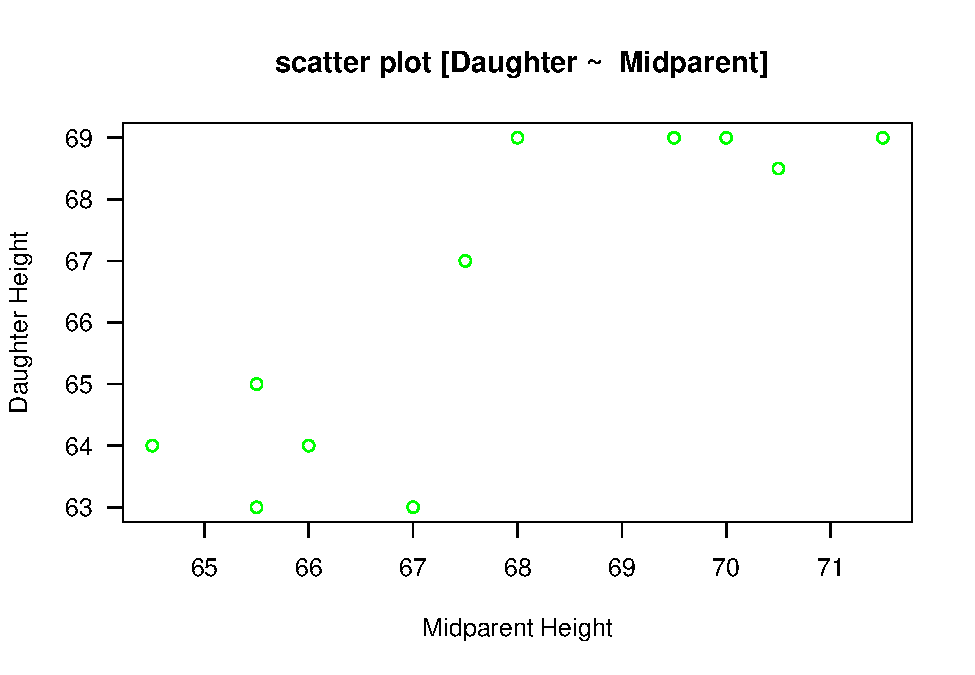
\includegraphics{OBLIG2-STAT111_files/figure-latex/unnamed-chunk-1-1.pdf}

Plottet hvis vi ser bort fra regresjons linjen kan intuitivt se ut som
at samler seg i venstre nedre hjørne

\end{document}
